Um quebra-cabe�a consiste em recobrir um quadrado com tri�ngulos ret�ngulos is�sceles, como ilustra a figura.

\begin{figure}[h]
\centering
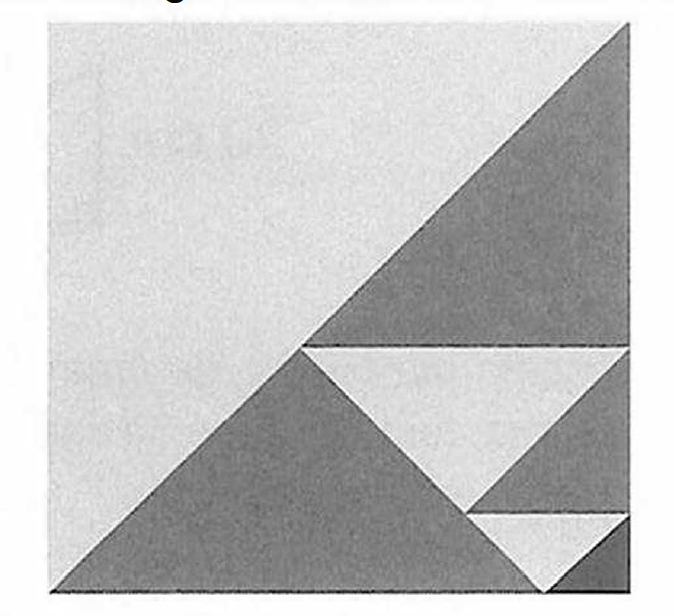
\includegraphics[width=8cm]{../figuras/q175-2018.png}
\end{figure}

Uma artes� confecciona um quebra-cabe�a como o descrito, de tal modo que a menor das pe�as � um tri�ngulo ret�ngulo is�sceles cujos catetos medem 2 cm.

O quebra-cabe�a, quando montado, resultar� em um quadrado cuja medida do lado, em cent�metro, � 

\begin{enumerate}
\item[a)]14
\item[b)]12
\item[c)]$7\sqrt 2$
\item[d)]$6+4\sqrt 2$
\item[e)]$6+2\sqrt 2$
\end{enumerate}